% Options for packages loaded elsewhere
\PassOptionsToPackage{unicode}{hyperref}
\PassOptionsToPackage{hyphens}{url}
\PassOptionsToPackage{dvipsnames,svgnames*,x11names*}{xcolor}
%
\documentclass[
  12pt,
]{article}
\usepackage{lmodern}
\usepackage{amssymb,amsmath}
\usepackage{ifxetex,ifluatex}
\ifnum 0\ifxetex 1\fi\ifluatex 1\fi=0 % if pdftex
  \usepackage[T1]{fontenc}
  \usepackage[utf8]{inputenc}
  \usepackage{textcomp} % provide euro and other symbols
\else % if luatex or xetex
  \usepackage{unicode-math}
  \defaultfontfeatures{Scale=MatchLowercase}
  \defaultfontfeatures[\rmfamily]{Ligatures=TeX,Scale=1}
\fi
% Use upquote if available, for straight quotes in verbatim environments
\IfFileExists{upquote.sty}{\usepackage{upquote}}{}
\IfFileExists{microtype.sty}{% use microtype if available
  \usepackage[]{microtype}
  \UseMicrotypeSet[protrusion]{basicmath} % disable protrusion for tt fonts
}{}
\makeatletter
\@ifundefined{KOMAClassName}{% if non-KOMA class
  \IfFileExists{parskip.sty}{%
    \usepackage{parskip}
  }{% else
    \setlength{\parindent}{0pt}
    \setlength{\parskip}{6pt plus 2pt minus 1pt}}
}{% if KOMA class
  \KOMAoptions{parskip=half}}
\makeatother
\usepackage{xcolor}
\IfFileExists{xurl.sty}{\usepackage{xurl}}{} % add URL line breaks if available
\IfFileExists{bookmark.sty}{\usepackage{bookmark}}{\usepackage{hyperref}}
\hypersetup{
  pdftitle={Statistical Learning Project},
  pdfauthor={1st Milestone},
  colorlinks=true,
  linkcolor=cyan,
  filecolor=Maroon,
  citecolor=Blue,
  urlcolor=magenta,
  pdfcreator={LaTeX via pandoc}}
\urlstyle{same} % disable monospaced font for URLs
\usepackage[margin= 2 cm]{geometry}
\usepackage{graphicx,grffile}
\makeatletter
\def\maxwidth{\ifdim\Gin@nat@width>\linewidth\linewidth\else\Gin@nat@width\fi}
\def\maxheight{\ifdim\Gin@nat@height>\textheight\textheight\else\Gin@nat@height\fi}
\makeatother
% Scale images if necessary, so that they will not overflow the page
% margins by default, and it is still possible to overwrite the defaults
% using explicit options in \includegraphics[width, height, ...]{}
\setkeys{Gin}{width=\maxwidth,height=\maxheight,keepaspectratio}
% Set default figure placement to htbp
\makeatletter
\def\fps@figure{htbp}
\makeatother
\setlength{\emergencystretch}{3em} % prevent overfull lines
\providecommand{\tightlist}{%
  \setlength{\itemsep}{0pt}\setlength{\parskip}{0pt}}
\setcounter{secnumdepth}{-\maxdimen} % remove section numbering
\usepackage{bbold}
\usepackage{mdframed, xcolor}
\usepackage{graphicx}
\mdfsetup{frametitlealignment=\center}
\usepackage{multirow}
\usepackage{enumitem}
\definecolor{shadecolor}{rgb}{0.89,0.8,1}
\newcommand{\Prob}{\mathbb{P}}
\newcommand{\Exp}{\mathbb{E}}
\newcommand{\Var}{\mathbb{V}\mathrm{ar}}
\newcommand{\Cov}{\mathbb{C}\mathrm{ov}}
\newcommand{\blue}{\textcolor{blue}}
\newcommand{\darkgreen}{\textcolor[rgb]{0,.5,0}}
\newcommand{\gray}{\textcolor[rgb]{.3,.3,.3}}
\newcommand{\blueA}{\textcolor[rgb]{0,.1,.4}}
\newcommand{\blueB}{\textcolor[rgb]{0,.3,.6}}
\newcommand{\blueC}{\textcolor[rgb]{0,.5,.8}}
\newcommand{\evidenzia}{\textcolor[rgb]{0,0,0}}
\newcommand{\nero}{\textcolor[rgb]{0,0,0}}
\newcommand{\darkyel}{\textcolor[rgb]{.4,.4,0}}
\newcommand{\darkred}{\textcolor[rgb]{.6,0,0}}
\newcommand{\blueDek}{\textcolor[rgb]{0.6000000, 0.7490196, 0.9019608}}
\newcommand{\purpLarry}{\textcolor[rgb]{0.6901961, 0.2431373, 0.4784314}}
\newcommand{\lightgray}{\textcolor[rgb]{.8,.8,.8}}
\newcommand{\bfun}{\left\{\begin{array}{ll}}
\newcommand{\efun}{\end{array}\right.}

\title{Statistical Learning Project}
\author{1st Milestone}
\date{G08}

\begin{document}
\maketitle

\hypertarget{prediction-and-analysis-of-air-quality}{%
\section{Prediction and analysis of air
quality}\label{prediction-and-analysis-of-air-quality}}

Riccardo Ceccaroni, Giusy Beatrice Colarusso, Gabriele Giannotta,
Francesco Lauro

\hypertarget{abstract}{%
\subsection{Abstract}\label{abstract}}

L'inquinamento atmosferico è uno dei grandi problemi che affligge le
aree metropolitane di tutto il mondo. Il traffico e le industrie
svolgono un ruolo significativo. Abbiamo bisogno di implementare modelli
che registrino informazioni sulle concentrazioni di inquinanti
atmosferici (\(SO_2\), \(NO_2\), ecc.) poichè la deposizione di questi
gas nocivi nell'aria sta influenzando la qualità della vita delle
persone.

La crescita della disponibilità di dati e l'avanzamento delle tecnologie
computazionali stanno rendendo possibile la previsione e l'analisi della
qualità dell'aria, fornendo informazioni estremamente utili per
controllare l'inquinamento atmosferico.

\hypertarget{main-research-aim-framework}{%
\subsection{Main research aim \&
framework}\label{main-research-aim-framework}}

Lo scopo principale del progetto è trovare il modello migliore che
riesca a predire la qualità dell'aria. I dati raccolti e l'analisi è
relativa alla zona \_\_\_\_.

L'interesse in questo argomento nasce dal fatto che pensiamo sia
importante conoscere la situazione della qualità dell'aria e che grazie
a delle previsioni sarebbe possibile controllare e forse ``ridurre''
l'inquinamento.

Un secondo obiettivo di questa ricerca, trovandoci in un periodo storico
``particolare'', ovvero la pandemia del Covid-19, è capire se
quest'ultima oltre a cambiare le nostre abitudini abbia avuto o meno
influenza sulla qualità dell'aria.

\hypertarget{data-sources}{%
\subsection{Data source(s)}\label{data-sources}}

I dati verranno presi giornalmente (4 misurazioni circa) dal sito
\href{https://aqicn.org/api/}{Air Quality Programmatic APIs} e
collezionati in un dataframe tramite uno
\href{https://github.com/ceccaroni1884368/SL_Project}{script} python da
noi sviluppato. Lo script si collega al sito tramite apposite API, fa
richiesta della qualità dell'aria di ogni stazione \_\_\_\_\_ messa in
lista ed inserisce le risposte in un dataframe che poi viene salvato in
formato \textit{.csv}. I dataframe di ogni osservazione verranno in
seguito uniti.

\hypertarget{data-collection}{%
\subsection{Data collection}\label{data-collection}}

Di ogni stazione dell'aria raccoglieremo i seguenti dati: data, ora,
località, indice \(AQI\), monossido di carbonio \(CO\), diossido di
azoto \(NO_2\), ozono \(O_3\), anidride solforosa \(SO_2\), particulate
matter \(PM_{10}\), particulate matter \(PM_{2.5}\), umidità \(h\),
pressione \(p\), temperatura \(t\) e velocità del vento \(w\).

Il problema principale nella raccolta dati risiede nel fatto che le
stazioni vengono aggiornate in orari diversi ed alcune vengono
aggiornate soltanto una volta al giorno. Per questo motivo potremmo
raccogliere più dati giornalieri di una stazione rispetto ad un'altra.

\hypertarget{model-methods}{%
\subsection{Model \& Methods}\label{model-methods}}

I due modelli che vorremmo testare su i dati raccolti sono:

\begin{enumerate}
\def\labelenumi{\arabic{enumi}.}
\item
  \textbf{Multiple Additive Regression Trees}: a machine learning
  technique for regression and classification problems, which produces a
  prediction model in the form of an ensemble of weak prediction models,
  typically decision trees (Wikipedia 2020b), (Karimian et al. 2019).
\item
  \textbf{ARIMA Model}: a generalization of an autoregressive moving
  average (ARMA) model. Both of these models are fitted to time series
  data either to better understand the data or to predict future points
  in the series (Wikipedia 2020a), (Bhalgat, Bhoite, and Pitare 2019).
\end{enumerate}

\hypertarget{softwarehardware-toolkit}{%
\subsection{Software/Hardware Toolkit}\label{softwarehardware-toolkit}}

In questo momento l'unico linguaggio di programmazione che abbiamo
utilizzato è stato \textit{Python}.

Per l'analisi dei dati continueremo ad utilizzare \textit{Python}
insieme ad \textit{R}. Molto probabilmente faremo uso dei pacchetti
\href{https://cran.r-project.org/web/packages/gbm/gbm.pdf}{gbm} e
\href{https://stat.ethz.ch/R-manual/R-devel/library/stats/html/stats-package.html}{stats}.

\hypertarget{project-timeline}{%
\subsection{Project Timeline}\label{project-timeline}}

\begin{center}
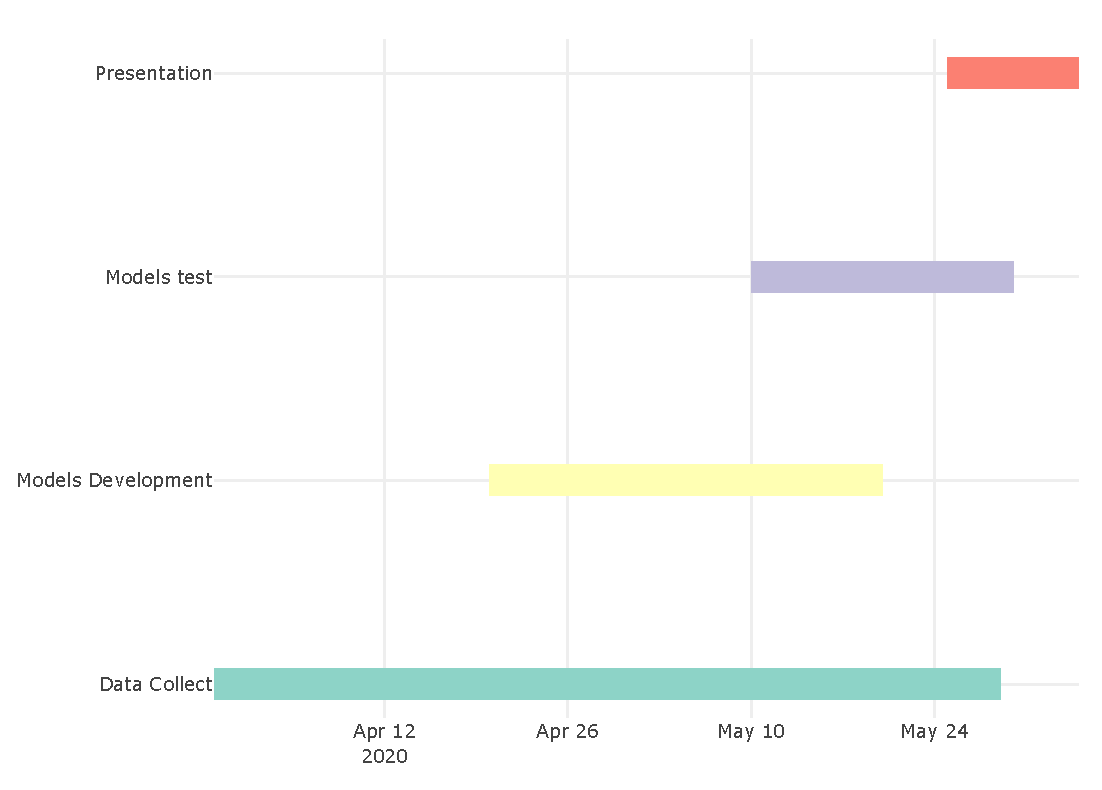
\includegraphics[height=9cm]{timeline.pdf}
\end{center}

\hypertarget{references}{%
\subsection*{References}\label{references}}
\addcontentsline{toc}{subsection}{References}

\hypertarget{refs}{}
\leavevmode\hypertarget{ref-article4}{}%
Bhalgat, Pooja, Sachin Bhoite, and Sejal Pitare. 2019. ``Air Quality
Prediction Using Machine Learning Algorithms.'' \emph{International
Journal of Computer Applications Technology and Research} 8 (September).
\url{https://doi.org/10.7753/IJCATR0809.1006}.

\leavevmode\hypertarget{ref-article3}{}%
Delavar, Mahmoud, Amin Gholami, Gholam Shiran, Yousef Rashidi, Gholam
Nakhaeizadeh, Kurt Fedra, and Smaeil Afshar. 2019. ``A Novel Method for
Improving Air Pollution Prediction Based on Machine Learning Approaches:
A Case Study Applied to the Capital City of Tehran.'' \emph{ISPRS
International Journal of Geo-Information} 8 (February): 99.
\url{https://doi.org/10.3390/ijgi8020099}.

\leavevmode\hypertarget{ref-article7}{}%
Karimian, Hamed, Qi Li, Chunlin Wu, Yanlin Qi, Yuqin Mo, Gong Chen,
Sonali Sachdeva, and Xianfeng Zhang. 2019. ``Evaluation of Different
Machine Learning Approaches in Forecasting Pm2.5 Mass Concentrations.''
\emph{Aerosol and Air Quality Research} 19 (January).
\url{https://doi.org/10.4209/aaqr.2018.12.0450}.

\leavevmode\hypertarget{ref-article5}{}%
Kleine Deters, Jan, Rasa Zalakeviciute, Mario Gonzalez, and Yves
Rybarczyk. 2017. ``Modeling Pm 2.5 Urban Pollution Using Machine
Learning and Selected Meteorological Parameters.'' \emph{Journal of
Electrical and Computer Engineering} 2017 (June): 1--14.
\url{https://doi.org/10.1155/2017/5106045}.

\leavevmode\hypertarget{ref-article6}{}%
Qi, Zhongang, Tianchun Wang, Guojie Song, Weisong Hu, Xi Li, Zhongfei,
and Zhang. 2017. ``Deep Air Learning: Interpolation, Prediction, and
Feature Analysis of Fine-Grained Air Quality.'' \emph{IEEE Transactions
on Knowledge and Data Engineering} PP (November).
\url{https://doi.org/10.1109/TKDE.2018.2823740}.

\leavevmode\hypertarget{ref-article2}{}%
Venegas, Laura, Nicolás Mazzeo, and Mariana Dezzutti. 2014. ``A Simple
Model for Calculating Air Pollution Within Street Canyons.''
\emph{Atmospheric Environment} 87 (April): 77--86.
\url{https://doi.org/10.1016/j.atmosenv.2014.01.005}.

\leavevmode\hypertarget{ref-article1}{}%
Wang, Ping, Yong Liu, Zuodong Qin, and Guisheng Zhang. 2014. ``A Novel
Hybrid Forecasting Model for Pm10 and So2 Daily Concentrations.''
\emph{The Science of the Total Environment} 505C (November): 1202--12.
\url{https://doi.org/10.1016/j.scitotenv.2014.10.078}.

\leavevmode\hypertarget{ref-wiki:Autoregressive_integrated_moving_average}{}%
Wikipedia. 2020a. ``Autoregressive integrated moving average ---
Wikipedia, the Free Encyclopedia.''
\url{http://en.wikipedia.org/w/index.php?title=Autoregressive\%20integrated\%20moving\%20average\&oldid=944420432}.

\leavevmode\hypertarget{ref-wiki:Gradient_boosting}{}%
---------. 2020b. ``Gradient boosting --- Wikipedia, the Free
Encyclopedia.''
\url{http://en.wikipedia.org/w/index.php?title=Gradient\%20boosting\&oldid=947218348}.

\end{document}
